\documentclass[a4paper,UKenglish]{lipics-v2018}
\usepackage{microtype}%if unwanted, comment out or use option "draft"
\bibliographystyle{plainurl}

\title{Formal Methods for Security - Final Report}

\author{Daniel Schaefer}{2549458}{}{}{}
\authorrunning{Daniel Schaefer}
\renewcommand{\copyrightline}{}

\def\murphi{Mur$\phi$ }

\begin{document}
\maketitle

\begin{abstract}
In this course we generally talked about various methods of model-checking security protocols. Later on here should be a text that summarizes the idea and findings of the seminar.\\
% TODO Extend

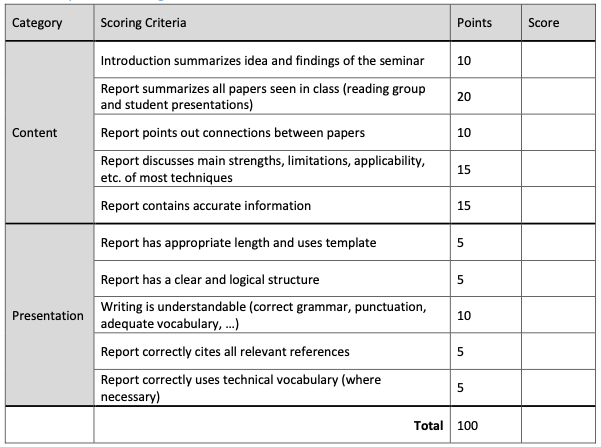
\includegraphics[scale = 0.72]{pictures/grading_scheme}\\
\end{abstract}


\newpage
\section{Model Checking Security Protocols}

This paper written by Basin et al. outlines the difficulties of analyzing a security protocol in an automated fashion. The hardness of this particular problem specifically originates from the non-deterministic adversary, that is able to interact with arbitrary many protocol-executions that are being interleaved. Interaction with the executions in this case means, that the adversary is in control of the network that the protocol is executed on, which means that it can intercept, redirect and alter any data that is being sent.\cite{model_checking_security_protocols}

Such an attacker model is also called the Dolev-Yao attacker model.  Many approaches of model checking cryptographic protocols adopted this attacker model and use it as part of an approach called 'Dolev-Yao symbolic model', which is explained in detail by Basin et al. in chapter 24.3.\cite{model_checking_security_protocols} 

In a symbolic model, messages are being represented by terms which formulate certain assumptions, essentially defining constraints on variables instead of arguing about concrete values. This measure is taken to counter the problem of state space explosion which is a consequence of the interleaving of protocol executions combined with the nondeterministic adversary. Clearly, these properties cause the statespace to be generally infinite.\cite{model_checking_security_protocols}

During et al. were able to proof that the secrecy problem of a security protocol is undecidable for such an attacker model if the number of protocol executions and random values (nonces) are unbounded.\cite{DLMS99} If one is able to keep the number of protocol executions bounded the secrecy problem was proven to be NP-complete by Rusinowitch and Turuani.\cite{RT01} This proof motivated development of model checkers in which the user explicitly specifies the number of protocol executions the model checker should search through which are in fact still useful in practice as most attacks on realistic protocols only require a few sessions.\cite{model_checking_security_protocols}

Still, this has to be considered a limitation as there might be attacks in practice which require the interleaving of a larger number of instances. Generally this publication outlines, that it is already hard to define a security property that is being satisfied, will not limiting the programs usefullnes for legitimate users.

Overall this paper summarizes a large number of important terms, security properties and other definitions that are helpful, specifically regarding to the application of model checking on security protocols. Later chapters provide examples of practical applications of such techniques using a variety of different ideas, including outlines of promising approaches for the future.

% TODO: MAYBE: Pick important parts of definitions and list them here or a bit later maybe

% TODO: MAYBE: Define State space explosion?

% TODO: MAYBE: explain Notion of Secrecy and Weak Aliveness
% TODO: MAYBE: Forward vs Backwards Search?
% TODO: MAYBE: Link to computational soundness
% TODO: MAYBE: Non-Trace properties: e.g. non-interference, observational equivalence



\newpage
\section{Language Based Information Flow Security}

Sabelfeld et al. explain a promising new approach to guarantee that secret input data is not being 'leaked' to an attacker which observes the system's output. This language-based technique, working on program semantics and analysis, relies on enforcing information-flow policies in source-code. Goal of these policies is to achieve properties like data confidentiality and noninterference.\cite{language_based_information_flow_security}

The approach, called "Information-flow control" is a mechanism to enforce such policies. The analysis that is performed must then proof that no information flow exists, that would violate the previously specified policies.\cite{language_based_information_flow_security}

There are a significant number of channels one could leak information over, which are not directly transfering data. An example for such channels would be "termination channels" and "timing channels", which are related to an attackers ability to observe the behaviour of the program execution additionally to its output. This means that e.g. the duration of an computation or the non-termination of the program might leak information about secret values that were used as part of these computations.
The same applies to a number of additional channels, which are also not used to transfer data but still offer possible information leaks.\cite{language_based_information_flow_security} % TODO: List other Covert Channels

The focus of this paper is on a type checking approach to perform static information-flow analysis at compile time. Such an approach has already been implemented in the Jif compiler for Java.\cite{JFlow} The general idea is that a \textit{security type} is assigned to every program expression. This security type contains the ordinary type of the expression (such as int, float, string, etc.) and additionally a static label which describes how the resulting value can be used. This value is static and not determined on runtime, such that it can be used to verify the control flow on compile-time already.\cite{language_based_information_flow_security}
To be able to track implicit flows correctly, dependencies of the program-counter are additionally tracked.

The advantage of performing verification on compile time, compared to checking during runtime is that one is not limited to a single program execution, instead one can proof security of all possible program paths.\cite{language_based_information_flow_security} Additionally such an approach solves the problem of expressing end-to-end security policies, which is currently a problem research is facing. Unfortunatly there are still some problems that have to be overcome, mainly related to the lack of expressiveness of current security-type systems and the need of semantics for embedded or concurrent systems. Generally these type-systems are quite hard to extend and the soundness proof would have to be repeated for every extension.\cite{language_based_information_flow_security}

This publication serves as an overview of current research in the field of information flow security with a focus on static analysis. The first paper already mentioned such an approach as a possible alternative, which is for example used by the AVISPA tool.\cite{model_checking_security_protocols} 



% TODO: second half of this paper basically not contained in this summary
% TODO: Problems with this paper/approach



\newpage
\section{Secure Information flow by self-composition}

Type systems are a way to enforce secure information flow of a program but are generally hard to extend, which is particularly disadvantagous when additions have to be made to verify a new security policy. This was one of the problems the previously presented publication by Sabelfeld et al. was still facing.\cite{language_based_information_flow_security} 

An alternative to these type systems is to use a more flexible approach of program logics, which this publication focuses on. Barthe et al. build on to the idea of self-composition, which reduces the problem to a safety property of the composition of a program with itself. Self-composition is essentially composing the program $P$ with a renaming of itself, resulting in a new program $Q$.
\cite{information_flow_by_self_composition}

Information flow properties are properties that correspond to at least two execution traces and can not be represented directly by a safety property. To overcome this problem, Barthe et al. were able to proof that non-interference of some program $P$ can be reduced to a property about every single program execution of a new program $Q$ that can be constructed using $P$ and a renaming of $P$, using the above mentioned approach of self-composition.\cite{information_flow_by_self_composition}
% TODO: paragraph above maybe to close to paper wording?

This reduction opens up a new way to apply (sound) programming logics to characterise non-interferance in an alternative way using this constructed program $Q$. This approach additionally allows a user to specify that some information can be leaked without violating the safety property immediately by defining the so called indistinguishability relation accordingly. This relation intuitively defines, which outputs should be considered equal or different, which affects the attackers ability to distinguish them. There are many cases in which such\textit{minor information leaks} are necessary to maintain the usefulness of a program.\cite{information_flow_by_self_composition}

A problem of the approach that was presented in this paper, is the limitation to abstract values of variables\cite{information_flow_by_self_composition}, which means that one can not perform any operations on pointer-types. This implies that control-flow of a program can not depend on memory allocation. It remains to be seen if this limitation can be overcome by extending the presented approach or by translating these cases into an equivalent form using only abstract values.

Still, the approach has to be considered very flexible as it can be used to proof a variety of policies without proving soundness repeatedly. Especially compared to security-type systems this is a clear advantage.

% TODO: explain self-composition here more, how the Program is built from P and P'









\newpage
\section{Automated Analysis of Cryptographic Protocols using \murphi}

\murphi is a tool to analyze cryptographic protocols using a state enumeration approach. In a feasibility study it was able to outperform similar finite-state exploration tools on the protocols that were tested. Notable difference were the more efficient approach of \murphi to counteract the State-space explosion problem and the ability to set interrupt points to guide the search by hand, which can also be helpful to work around the State-space explosion problem.\cite{murphi}

\murphi performs explicit state enumeration using either breadth-first or depth-first search to proof that all reachable states satisfy some specification that is given by the user. The protocol has to be specified using the \murphi language, which can be extended to contain additional information for an attacker such as leaking some supposedly secret values initially which would reflect the assumption that part of the system was compromised already. Due to the fact that \murphi performs explicit state enumeration, one has to limit the number of states, which is done by fixing system size parameters, such as the number of agents that perform the cryptographic protocol with each other. These limitations have to be specifially set by the user and \murphi is only able to guarantee correctness of this "down-scaled" version of the protocol. Clearly it is not trivial to set these numbers, as larger values often have exponential effect on the runtime of the tool.\cite{murphi} Regardless, it is an advantage that these bounds can easily be changed by a user.

Performance of \murphi is significantly improved using a hash table which stores the reached states as this avoids recomputation when visiting the same state again in the future. The memory used by this hash table is typically a limitation of the \murphi tool.\cite{murphi}
% TODO: maybe list other features that significantly improve performance, quite a lot of them

Formulating a protocol in the \murphi language reveals some issues a user might have. It is important to simplify to protocol and only modeling the key steps and primitives that are necessary to perform the protocol. This is particularly important to reduce the number of states that are explicitly enumerated. Additionally it is essential to define precisely which messages will be accepted or declined by each participant of the protocol and also how these messages are formated, because \murphi uses shared variables to communicate. These shared variables are accessable by an attacker, which is part of the ability of a Dolev-Yao attacker (network under control of adversary).\cite{murphi}

Similar issues arise when formulating an adversary to a protocol. The user has to specify the entire knowledge of the adversary and a finite set of actions that the adversary could perform at any point in time depending on the knowledge the adversary has gathered until this point.\cite{murphi}

% TODO: IMPORTANT: explain when/how 'wrong' error traces occur and how one specifies protocol/attacker around these

% TODO: maybe list problems/results from modeling the protocols that are listed throughout the entire paper




\newpage
\section{SAT based model-checking for security protocol analysis}

This approach interprets violations of a protocol as reachability problens, which means that one can apply any SAT solver to solve this issue efficietly. To achieve this, one has to build a propositional formula which models possible attacks on the protocol. If the SAT solver that is used to check this propositional formula for satisfiability is able to find a solution, this solution specifies an attack on the protocol and the protocol was proven to be insecure for the specified bounds.\cite{sat}

A significant advantage of using a SAT solver as a blackbox to verify the security of a protocol, is that all improvement in the field of SAT solvers can be equally used to enhance this approach. The already very efficient modern SAT solvers lead to very promising results in the experimental protocol verification that was performed by Armando etl al. Their approach already achieved similar performance than state of the art alternatives.\cite{sat}

The specification of possible attacks on the protocol that leads to the propositional formula is performed by using a framework based on multi-set rewriting. The number of sessions has to be bounded, such that the problem remains decidable.\cite{sat}

% TODO: page 4 left side upper 1/3, it sounds almost like this bound does not change much, because there is always a bound k that it can be safely reduced to

The authors provide semantics to perform this multi-set-rewriting to generate the propositional formula. They additionally developed an approach of how to safely eliminate non-determinism, which is e.g. associated with the generation of random values.
Encoding techniques that were originally developed for planning to security protocols were adapted to be applicable to increase efficiency of the formula generation. Armando et al. were able to proof both soundness and completeness of this modified approach.\cite{sat}

Conducted experiments indicated that the resulting formula scales better with a large number of agents and sessions, but worse with an increased message size, when compared to current state-of-the-art alternatives.\cite{sat}


% TODO: mention maybe future extension to LTL



\newpage
\section{Automatic Verification of Security Protocols in the Symbolic Model: the Verifier ProVerif}

Proverif is a Verifier that works in the symbolic model, which makes it easier to perform fully automatic verification. A special property of this verifier is that it is able to verify protocols assuming an unbounded number of protocol executions. Because this is a generally undecidable problem, Proverif can not guarantee termination in all cases.\cite{ProVerif}

The protocol has to be specified in an extension of the pi calculus, which already supports a wide variety of cryptographic primitives out of the box. On this protocol, Proverif is able to proof a variety of security properties such as for example secrecy, authentication and some properties of observational equivalence.\cite{ProVerif}

Proverif's efficieny comes from the automatic translation into horn clauses. Not only the protocol itself is represented in these clauses, but rather the attacker combined with the protocol. One could say that proverif abstracts much further away from the actual protocol than most approaches we encountered in this seminar. The set of horn clauses is internally simplified using resolution and additional optimisations. Particularly the optimisations which are specific to protocols reduce the number of clauses very significantly. Bruno Blanchet was able to proof that all these approximations are sound, which is essential to their usage as part of a verifier. All these approximations result in Proverif being able to handle very complex protocols.\cite{ProVerif}

However there are a couple of tradeoffs, these approximations introduce. The two most impactful ones are, that the order of actions is abstracted entirely and that each action can be repeated an unbounded number of times at any later time. Particularly for protocols that contain temporary secrets, there is a possibility of Proverif outputting a false attack.
This means that one has to additionally double-check an attack that is output by Proverif for validity. \cite{ProVerif}

The ability to verify protocols without limitations on the number of sessions or the message size imply that Proverif is well suited to be used for the certification of protocols.\cite{ProVerif}


\newpage
\section{Secure Information Flow as a Safety Problem}

Aiken et. al. developed a framework which improves on traditional type-based approaches and works better than the standart self composition approach, as formulated by Barthe, D'Argenio and Rezk. The authors apply  self-composition approach with the addition of information downgrading.\cite{secure_information_flow_safety}

% TODO: cite Barthe D'Argentio and Rezk

It is important to note, that only deterministic programs are being considered in this publication. 

The authors were able to reduce an alternative definition of termination-insensitive Secure Information Flow to a safety problem by making use of self-composition as part of their reduction. According to the authors it would be relatively easy to define a similar property for termination sensitive secure information flow using a liveness property.\cite{secure_information_flow_safety}

To overcome the limitation of Secure Information Flow being considered too strict for many applications, Aiken et. al. introduced the ability to downgrade information, inspired by Barthe, D'Argenio and Rezk. Output is then allowed to depend on the downgraded parts of high variables, which can e.g. be used to leak the length of some secret information while still keeping the secret information itself unknown.\cite{secure_information_flow_safety}

Unfortunatly, the self-composition approach seems to be too inefficient in practice, even combined with state-of-the-art safety analysis tools like BLAST. According to the authors of this publication it seems unlikely that any future advances in this field will change that.\cite{secure_information_flow_safety}

To overcome the issues of self-composition, Aiken et. al. first apply a type-directed transformation, which depends on a type system and outputs a program that is equivalent to the self-composition of the initial program. A specific type system for this usecase can be used to simplify the output program while maintaining important properties for safety analysis. This relatively inexpensive transformation causes the programs to be more digestible for the analysis tools, which makes is a clear  improvement on the type-based approach.\cite{secure_information_flow_safety}

% TODO: Section 3


\newpage
\section{Automatic Discovery and Quantification of Information Leaks}

Backes et al. developed an approach to not only discover information leaks but additionally specify which information is leaked and quantify that information leak.\cite{automatic_discovery_and_quantification}

Their solution provides the number of discovered equivalence classes and their respective sizes, without having to specify the equivalence relation manually. While existing qualitative approaches are able to e.g. determine the number of secret bits that are leaked, they do not provide a comprehensive measure to establish security guarantees.\cite{automatic_discovery_and_quantification}

The approach described in this publication starts by using an initial candidate, which is assumed to be the equivalence relation. It then refines the relation step by step until no further leaks are found in the current equivalence relation. This problem is formulated as a reachability problem and solved by a model-checker, which is used as a blackbox.\cite{automatic_discovery_and_quantification}

The resulting equivalence relation essentially describes what an attacker can learn about the input of the program by observing the programs output behaviour. The cardinality of these classes can be computed using LATTE.\cite{automatic_discovery_and_quantification}

On the computed equivalence classes they apply Shannon Entropy, Guessing Entropy, Channel Capacity etc. to interpret the classes. This leads to easily human-readable metrics, such as the attackers uncertainty about the secret bits before and after a single guess.\cite{automatic_discovery_and_quantification}

A advantage of this approach is that while the used model-checkers are not complete, they are sound which means that they might introduce an over-approximation of information leakage, but never an under-approximation. This means that the described approach can be used to certify the security of a program.\cite{automatic_discovery_and_quantification} Clearly, the over-approximation can also be a disadvantage in some cases. 

Another limitation of the described algorithms, is that they assume the termination of the program on any provided input.

The experimental results contained in this publication should also be seen as an indicator that this approach might not be feasable in practice. Main reason for this is the runtime their algorithm takes even on simplified problems.\cite{automatic_discovery_and_quantification}


\newpage
\section{Verifying Constant-Time Implementations}

An entirely new attack vector, that is very hard to avoid entirely are so called timing attacks. Developing software which adheres to constant-time practices is not only very error-prone but also bottlenecks efficiency of software. In fact there have been a number of occasions were timing-based attacks were discovered on widely used software such as for example OpenSSL's RSA decryption.

% Maybe mention recent intel bugs with cache collisions here

Almeida et al. propose a new approach, called "ct-verif" to automatically verify whether  or not a timing attack is possible on the software that is being verified. In order to include most compiler-optimizations in their baseline of testing, their approach verifies LLVM assembly code, which also makes the approach easily transferable to all languages that can be compiled to LLVM assembly.\cite{verifying_constant_time_implementations}

A commonly used guideline to secure software against such kind of attacks is that branching never depends on program secrets in any way. An even stronger policy would be that accesses memory addresses, and their order of access do not depend on any secrets as well. Clearly programmers are forced to deviate from conventional practices to fullfill policies like these.\cite{verifying_constant_time_implementations}

The tool ct-verif is fully automatic after the user specified which inputs and outputs are public to an attacker. A program P's program paths are independant of all program-secrets if assertion-safety of a program Q that is essentially a product of the P with itself holds.\cite{verifying_constant_time_implementations} Clearly, the construction of Q is inspired by self-composition. 

Almeida et al. additionally provided a proof in Coq, which verified this reduction to be both sound and complete.\cite{verifying_constant_time_implementations}

Additionally Almeida et al. provided a formalization of constant-time theory, which provides a foundation for constant-time policies used in practice.

It was demonstrated on examples such as OpenSLL, NaCl, FourQlib and others, which supported the practical effectiveness of ct-verif. Overall the case study showed, that ct-verif is able to validate significantly more constant-time programs than the previously existing tools.\cite{verifying_constant_time_implementations}

A potential problem of this approach is that it works on LLVM assembly, instead of machine code and while the LLVM assembly might fullfill the desired constant time policy, it is not entirely clear wheather this also holds for the resulting machine code in all cases.\cite{verifying_constant_time_implementations}



\newpage
\bibliography{finalReport}


\end{document}